\documentclass[a4paper,10pt]{article}
\usepackage[utf8]{inputenc}
\usepackage{amsmath}
\usepackage{graphicx}
\usepackage{epsfig}
\usepackage[english]{babel}
\usepackage{url}
\usepackage{epstopdf}
\usepackage{subfig}
\usepackage{graphicx}
\usepackage{enumerate}
\usepackage{appendix}
%\usepackage{anysize}
%\marginsize{1cm}{1cm}{1cm}{1cm}
\title{\textit{IEE3853} Detectores para Astronomía (I-2012)}
\author{\textbf{Tarea 04 – Diseño del sistema de detección para un Imager} \\Norman F. Sáez\\nfsaez@uc.cl}

\date{2012/07/07}

\begin{document}
%\input{portada}
\maketitle
\section*{Introducción}

El presente documento especifica sistema de detección para el telescopio ESO 1
metro, en donde el instrumento a utilizar es Imager Reducer.  Los requerimientos
son los siguientes:

\begin{itemize}
\item Especificar el CCD científico.

\item Predecir readout noise, dark current y readout time.

\item Estimar si el diseño óptico es adecuado o es preferible modificarlo, para
el detector seleccionado. En caso de modificación, especifique los
requerimientos para el nuevo diseño óptico.

\item Estimar los tiempos de exposición para diversos filtros considerando la
eficiencia cuántica del CCD seleccionado y la obtención de una SNR de al menos
10. Analice filtros del tipo SDSS4 (Sloan Digital Sky Survey) para su análisis.

\item Especificar los requerimientos de enfriamiento criogénico, en particular
temperatura de operación. Sugerir posibilidades de criogenia.
\end{itemize}

Las siguientes secciones intentan cumplir con las especificaciones de la tarea.


%PREGUNTA 1
\section{Especificación CCD a utilizar}
Parámetros del sistema:
\begin{itemize}
\item Field of View del instrumento = $14 '$
\item Diámetro Plano Focal = $30.8 [mm]$
\item Escala en el plano focal = $\frac{FoV}{Diametro\ Plano\ Focal} = 0.4545 ['/mm]$
\item Field of View requerido: $5'$ en x
\item Field of View requerido: $5'$ en y
\item Dimensiones del detector: $\frac{5'}{0.4545['/mm]} = 11 [mm]$ en x
\item Dimensiones del detector: $\frac{5'}{0.4545['/mm]} = 11 [mm]$ en y
\end{itemize}
Entonces el detector debe tener un tamaño de $11x11[mm]$.  Tamaño imagen de la
PSF en el plano focal: $\frac{0.00833'}{0.4545 ['/mm]} = 0.01833[mm] = 18.33516
[\mu m]$, utilizando el dato de Optimal Sampling, podemos obtener cuanto tiene
que ser el tamaño del píxel: $\frac{18.33516}{3} = 6.111 [\mu m]$.

Con los datos obtenidos, se necesita:
\begin{itemize}
\item $11x11[mm]$ como tamaño máximo del CCD.
\item Tamaño mínimo de cada píxel $6.11 [\mu m]$.
\end{itemize}

Con estas especificaciones no es posible obtener un CCD desde la página del
proveedor. Por lo que se intentara buscar uno similar y ajustar algunos
parámetros del instrumento.  Los datos obtenidos para determinar que no existe
un CCD que reúna las características adecuadas, se muestran en figura
\ref{fig:p1} 
\begin{figure}[ht!]
  \centering
  \subfloat[Tabla de datos siguiendo especificaciones]{\label{fig:p1_a}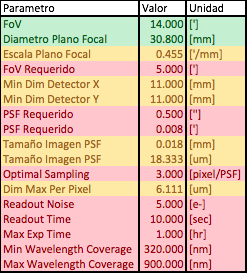
\includegraphics[width=0.5\textwidth]{img/img1}}
  ~ 
  \subfloat[Simbología]{\label{fig:p1_b}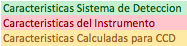
\includegraphics[width=0.3\textwidth]{img/simbologia}}
  ~ 
  \caption{Tabla de datos y simbología de acuerdo a las especificaciones}
  \label{fig:p1}
\end{figure}



%PREGUNTA 2
\section{Estimar si el diseño óptico es adecuado o es preferible
modificarlo,para el detector seleccionado. En caso de modificación, especifique
los requerimientos para el nuevo diseño óptico.} 

Dado que no existían CCD que se ajustaran a las especificaciones, se plantea la
siguiente solución:
\begin{itemize}
\item Disminuir escala en el plano focal del instrumento
\end{itemize}

Para ello, se necesita:
\begin{itemize}
\item Disminuir el Field of View.
\end{itemize}
o bien:
\begin{itemize}
\item Aumentar el diámetro.
\end{itemize}

Luego, se seleccionaron cámaras que tuvieran el diámetro focal cercano a 30.8.
Las mejores cámaras escogidas fueron:
\begin{itemize}
\item CCD42-40,  Image Area: 27.64x27.64 $[mm]$ ( o 764.411904 $[mm^2]$)
\item CCD55-30,  Image Area: 25.92x27.94 $[mm]$ ( o 724.3344   $[mm^2]$)
\item CCD230-42, Image Area: 30.96x30.72 $[mm]$ ( o 951.0912   $[mm^2]$)
\end{itemize}
Se estudia la opción de elegir CCD42-40 debido Field of View cercano a 30.8.
Para utilizar este detector, se tiene que ajustar el Field of View de las
especificaciones, de tal manera que sea coherente con el tamaño máximo que
pueden tener los píxeles.  Ver figura \ref{fig:ccd42p2} para revisar los datos
obtenidos.
\begin{figure}[ht!]
  \centering
  \subfloat[CCD42-40 Tabla de datos ajustando especificaciones]{\label{fig:ccd42p2_a}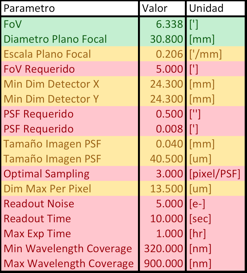
\includegraphics[width=0.5\textwidth]{img/ccd42-40}}
  ~ 
  \subfloat[Simbología]{\label{fig:ccd42p2_b}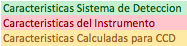
\includegraphics[width=0.3\textwidth]{img/simbologia}}
  ~ 
  \caption{CCD42-40}
  \label{fig:ccd42p2}
\end{figure}

Otra posibilidad es elegir CCD55-30. En este caso también es necesario
modificar el Field of View de acuerdo a las especificaciones del detector, al
igual que en CCD42-40.  Ver figura \ref{fig:ccd50p2} para revisar los
parámetros obtenidos.
\begin{figure}[ht!]
  \centering
  \subfloat[CCD55-30 Tabla de datos ajustando especificaciones]{\label{fig:ccd50p2_a}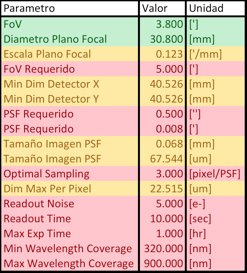
\includegraphics[width=0.5\textwidth]{img/ccd55-30}}
  ~ 
  \subfloat[Simbología]{\label{fig:ccd50p2_b}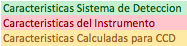
\includegraphics[width=0.3\textwidth]{img/simbologia}}
  ~ 
  \caption{CCD55-30}
  \label{fig:ccd50p2}
\end{figure}

La última opción a considerar es CCD230-42, debido a que su image view es
cercano a 30.8 y dentro de las CCD seleccionadas, es la que tiene mayor image
view. Se ajusta Field of View para que cumpla con las especificaciones del
detector  y también el diámetro en el plano focal. De acuerdo a las
especificaciones del CCD, se recalcula el Field of View para que cumpla los
valores tanto de tamaño de los píxeles así como el tamaño del CCD, y se aumenta
en 0.2[mm] el diámetro en el plano focal para calzar las especificaciones del
detector.  Ver figura \ref{fig:ccd230p2}, con los valores de los parámetros
obtenidos.
\begin{figure}[ht!]
  \centering
  \subfloat[CCD230-42 Tabla de datos ajustando especificaciones]{\label{fig:ccd230p2_a}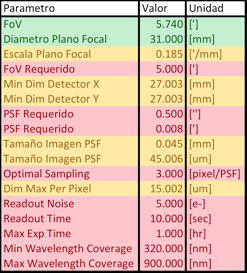
\includegraphics[width=0.5\textwidth]{img/ccd230-42}}
  ~ 
  \subfloat[Simbología]{\label{fig:ccd230p2_b}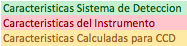
\includegraphics[width=0.3\textwidth]{img/simbologia}}
  ~ 
  \caption{CCD230-42}
  \label{fig:ccd230p2}
\end{figure}

Hasta el momento, se consideraran todos estos detectores como detectores
válidos, ya que para todos ellos hay que hacer modificaciones al diseño
original. En las siguientes preguntas, se intentara decir por la mejor opción
cumpliendo las características requeridas.
%PREGUNTA 3
\section{Predecir readout noise, dark current y readout time}
Dada las características presentadas en la pregunta 2 y el datasheet de cada
detector, se revisa a continuación spectral range, readout noise, dark current y readout
frequency, para cada caso:
\subsection{Spectral Range}
\begin{figure}[ht!]
  \centering
  \subfloat[Spectral range para todas las cámaras propuestas]{\label{fig:spectral}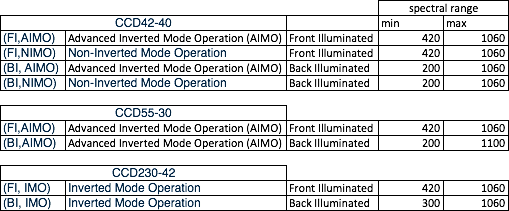
\includegraphics[width=0.8\textwidth]{img/spectral_range}}
  ~ 
  \caption{Spectral Range en $[nm]$}
  \label{fig:p3_b}
\end{figure}
Dada los requerimientos, solamente es posible utilizar detectores del tipo Back Illuminated.
%\newpage
\subsection{Readout Frequency}
Podemos estimar readout frequency de la siguiente manera:
\begin{description}
\item [pixels]: Número de píxeles total del CCD
\item [tiempo]: Máximo tiempo de lectura requerido
\item [amplificadores]: Número de amplificadores de salida
\end{description}

Dado los parámetros anteriores el readout frequency se puede calcular: 
\begin{align*}
readout\ frequency &= \frac{pixels}{tiempo*amplificadores}\\
\end{align*}
En figura \ref{fig:p3} están los resultados obtenidos para cada detector.
\begin{figure}[ht!]
  \centering
  \subfloat[CCD42-40]{\label{fig:ccd42p3}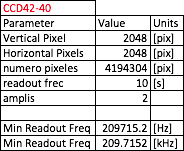
\includegraphics[width=0.3\textwidth]{img/ccd42-40p3}}
  ~ 
  \subfloat[CCD55-30]{\label{fig:ccd50p3}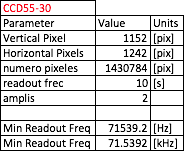
\includegraphics[width=0.3\textwidth]{img/ccd55-30p3}}
  ~ 
  \subfloat[CCD230-42]{\label{fig:ccd230p3}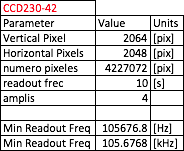
\includegraphics[width=0.3\textwidth]{img/ccd230-42p3}}
  ~ 
  \caption{Readout Frequency para cada detector}
  \label{fig:p3}
\end{figure}

\subsection{Readout Noise}
\begin{figure}[ht!]
  \centering
  \subfloat[Readout Noise para todas las cámaras propuestas]{\label{fig:readout}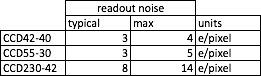
\includegraphics[width=0.4\textwidth]{img/readoutnoise}}
  ~ 
  \caption{Readout Noise}
  \label{fig:p3_a}
\end{figure}

Dada los requerimientos y en base a figura \ref{fig:p3_a}  no es posible
utilizar CCD230-42, debido a que supera el readout noise requerido, descartándola. 

\subsection{Dark Current}
Dark current para todos los detectores propuestas se puede revisar en \ref{fig:p3_c}
\begin{figure}[ht!]
  \centering
  \subfloat[Dark Current para todas las cámaras propuestas]{\label{fig:darkcurrent}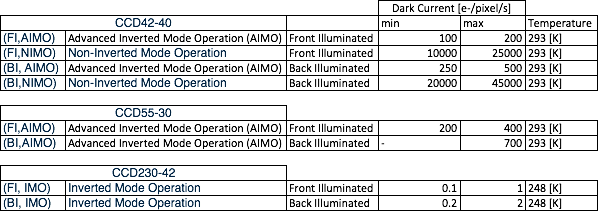
\includegraphics[width=0.8\textwidth]{img/darkcurrent}}
  ~ 
  \caption{Dark Current}
  \label{fig:p3_c}
\end{figure}

Cabe señalar que no es posible hacer una comparativa con todos los modelos,
debido a que cada una de las cámaras cambia dark current dependiendo de la
temperatura.

De acuerdo a los datos anteriores, se descarta CCD230-42, debido a su alto
readout noise. Además las características del tamaño del píxel requerido y las
modificaciones que se deberían hacer en el Field of View, impide la utilización
de CCD55-30 descartando este detector. \textbf{La mejor opción es CCD42-40}. El
Field of View es el mayor de todos y además Image Area es mayor a CCD55-30, su
mas cercano rival. A favor de CCD42-40 es el tamaño del píxel comparando con
CCD55-30. (CCD55-30 tiene un píxel de tamaño $\pm 22 [\mu m]$ comparado con el
tamaño del píxel de CCD42-40 que es de $\pm 15 [\mu m]$).

Cabe señalar que existen distintos tipos de CCD42-40 y la diferencia entre
ellas es la tecnología utilizada. Las tecnologías son:

\begin{itemize} 
\item Advanced Inverted Mode Operation (AIMO)
\item Non-Inverted Mode Operation (NIMO)
\end{itemize}

AIMO tiene 100-1000x dark current más bajo que NIMO, a la misma temperatura.
Si hay problemas para el enfriamiento, AIMO podría ser mejor. Es por esto que
se fabrican pocos modelos CCD42-40 NIMO. Por las razones anteriores, \textbf{se
decide utilizar tecnología AIMO}.

Luego de consultar directamente al proveedor (Alice Reinheimer
\url{alice.reinheimer@e2v-us.com}) sobre la disponibilidad de todos los
detectores CCD42-40 los detectores disponibles son los siguientes:

\begin{itemize} 
\item CCD42-40, AIMO, basic process, midband AR coated device.
\item CCD42-40, AIMO, basic process with broadband AR coating.
\end{itemize}

Se revisa cuidadosamente que tipo de coating cubre mejor las especificaciones
iniciales. Los gráficos adjuntos en figura \ref{fig:qe100} muestran Quantum
Efficiency a -100 grados celsius. En la figura \ref{fig:qe20} muestra Quantum
Efficiency a -20 grados celsius.

\begin{figure}[ht!]
  \centering
  \subfloat[QE v/s Wavelength, -100 C]{\label{fig:qe100a}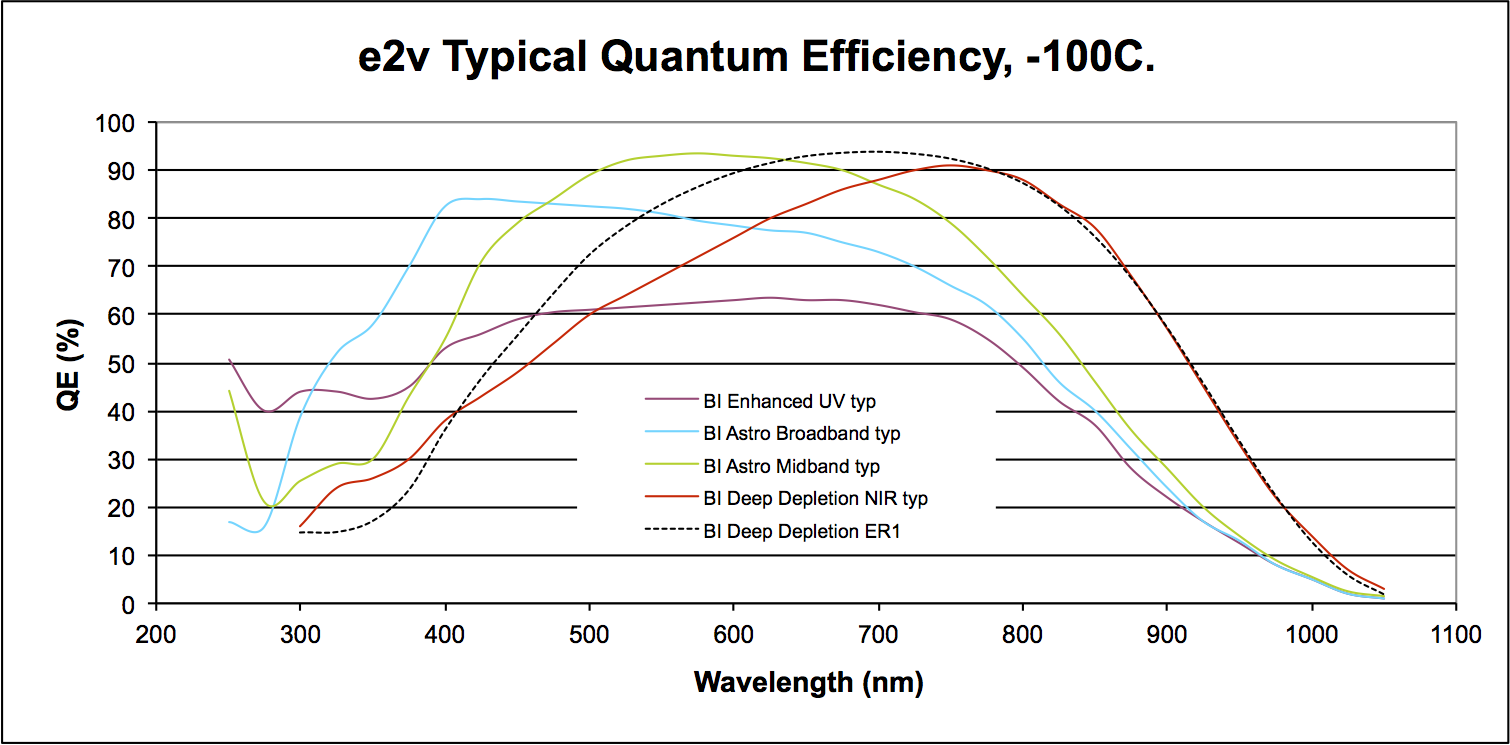
\includegraphics[width=0.9\textwidth]{img/qe100}}
  ~ 
  \caption{Quantum Efficiency (\%) v/s Wavelength ($[nm]$) , -100 [C], Back Illuminated}
  \label{fig:qe100}
\end{figure}

\begin{figure}[ht!]
  \centering
  \subfloat[QE v/s Wavelength, -20 C]{\label{fig:qe20a}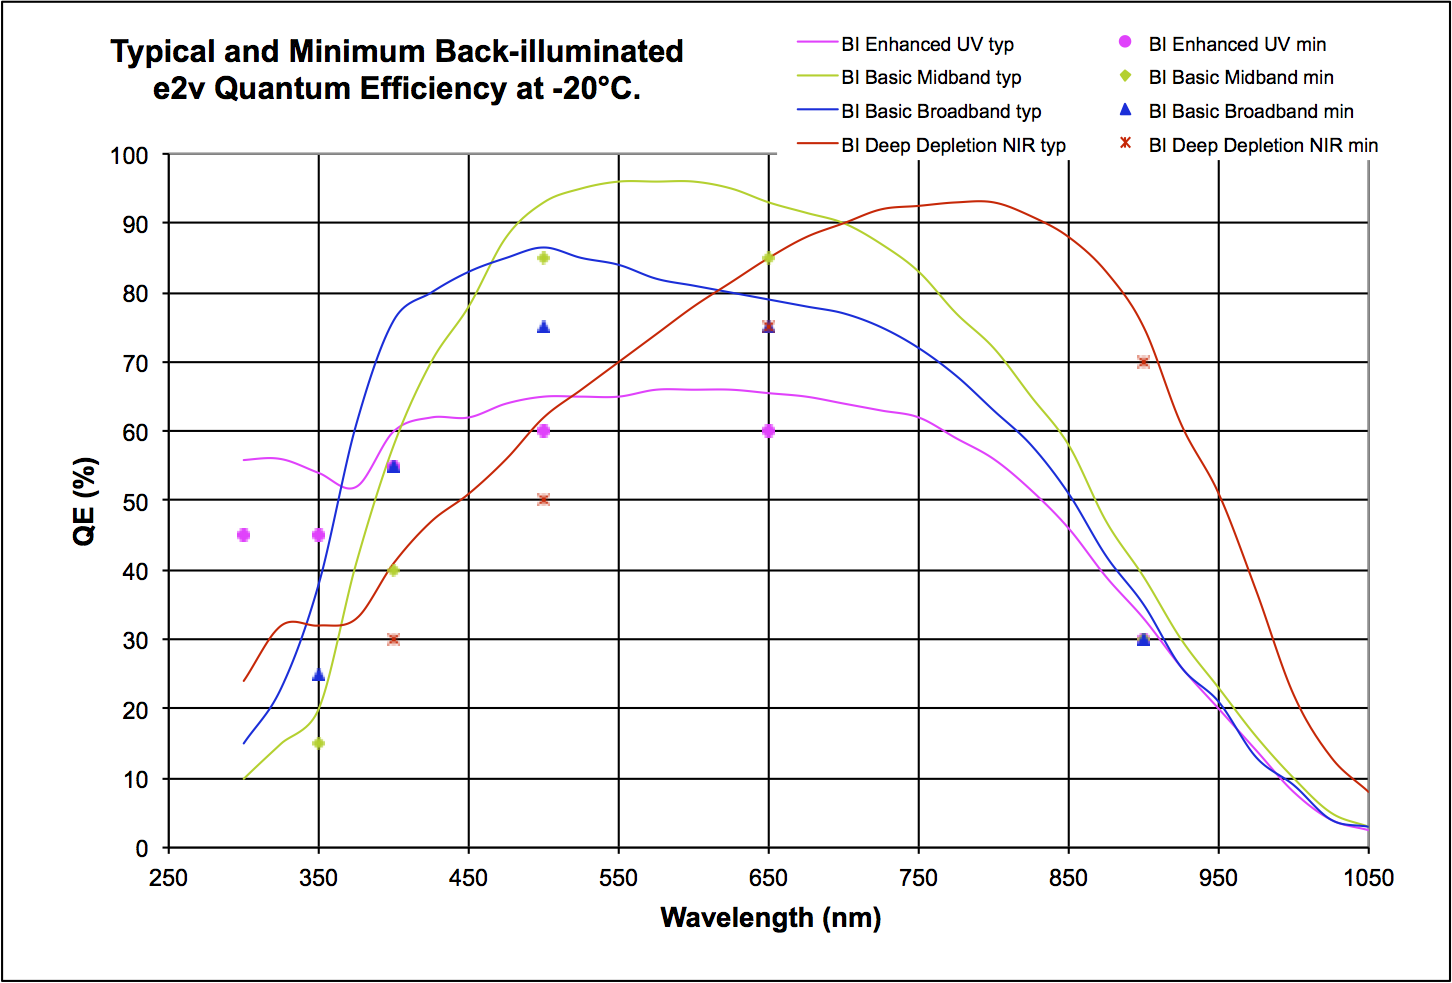
\includegraphics[width=0.9\textwidth]{img/qe20}}
  ~ 
  \caption{Quantum Efficiency (\%) v/s Wavelength ($[nm]$), -20 [C], Back Illuminated}
  \label{fig:qe20}
\end{figure}
 
Broadband coating es mejor para longitudes de onda entre 300 y 450 $[\mu m]$
sin embargo es peor desde 450 a 900 $[\mu m]$ comparado con midband. Debido a
que midband cubre un rango de longitud de onda mayor, \textbf{se prefiere
elegir  midband coating en desmedro de las longitudes de onda 300 a 450 $[\mu
m]$}. En las temperaturas -100 y -20 celsius,  se observa el mismo comportamiento. 
%PREGUNTA 4
\section{Estimar los tiempos de exposición para diversos filtros considerando la
eficiencia cuántica del CCD seleccionado y la obtención de una SNR de al menos
10. Analice filtros del tipo SDSS4 (Sloan Digital Sky Survey) para su análisis.}

Para poder analizar esta pregunta es necesario tener en consideración solamente CCD42-40, ver la figura \ref{fig:p4}

\begin{figure}[ht!]
  \centering
%  \subfloat[QE v/s Wavelength]{\label{fig:p4_a}\includegraphics[width=0.8\textwidth]{img/QE}}
  ~ 
  \caption{Quantum Efficiency (\%) v/s Wavelength ($[nm]$)}
  \label{fig:p4}
\end{figure}

%PREGUNTA 5
\section{Especificar los requerimientos de enfriamiento criogénico, en particular
temperatura de operación. Sugerir posibilidades de criogenia.}


\end{document}

